\subsection{Trust-Related Behaviors} \label{sec:trbs}
Something that is well accepted among researchers of all disciplines is that trust ultimately leads to some kind of behavior or action; this idea was highlighted by \citet{Lewis1985-pr}.  \citet{McKnight2001-fa} call these `trust-related behaviors` (TRBs), which is the term that will be used in this survey. In the case of a human-AIA relationship, the author is concerned with TRBs could include the kinds of tasks the human user assigns to the UGV such as accepting and following through on its plan, or directing that a new plan be made.

\subsubsection{Calibration of Trust-Related Behaviors}
    Trust is not a quantity that can be objectively measured. Rather, its relative magnitude must be observed through changes in TRBs, or qualitative surveys \cite{Muir1996-gt}. Of these two approaches, TRBs are the more objective measure due to the fact that people are not always consistent in their ratings, and may sincerely feel different levels of trust while performing similar TRBs. \citet{Parasuraman1997-co} were interested in understanding the use of automation by humans, and defined terms related to TRBs along these lines. Here it is proposed that, by extension, those terms also apply to the relationship between humans and AIAs. Within this scope the definitions are as follows\footnote{a third term `Abuse' was left out because it concerns the decision by humans to install automation in an environment that was inappropriate. It is my belief that this can be wrapped under the umbrella of `Misuse'},
    
    \begin{description}
        \item [Misuse:] The over-reliance on an AIA -- which could manifest itself in expecting too much accuracy from and AIA, or believing that it can be applied in an application that it was not designed to function in
        \item [Disuse:] The under-utilization of and AIA -- which could be manifest in a user turning off the AIA, or failing to use all of its capabilities 
        \item [\textbf{Abuse}:] I don't agree that abuse should be included -- we should talk about it
        % \item [Abuse:] Inappropriate application of automation (where \emph{application} in this case means the choice to deploy automation in a certain context, such as the choice to install a robot in a factory).
        % \nisarcomm{I don't think you should leave it out -- there is an important and subtle difference between over-reliance and misapplication of a capability/technology -- assurances to prevent the former are thus not going to be the same as assurances that try to avoid the latter. Also, the installation of automation in an environment that is inappropriate doesn't necessarily translate the same way to autonomous systems -- in particular, since autonomous systems often have to be self-directed and make decisions under uncertainty on their own. i.e. using the Google car to tow another vehicle behind it would not necessarily count as over-reliance/misuse, but could possibly be construed as abuse -- it is in the right environment, and it is still carrying out a function that any rational user might possibly conceive as a capability it ought to possess, since the car is still essentially carrying out the same function as before and doing what any car might be expected to do -- however, a user may not be aware of the fact that placing another vehicle in tow behind the car might introduce perception errors and planning errors, since the vehicle may not be able to fully account for the altered dynamics or changed sensor field, etc. -- it was not really designed for towing tasks, but someone might get lucky and get away with pulling it off a few times. In contrast, using the Tesla autopilot on the highway (even though it results in a crash while driver is watching a movie) is not abuse but clearly a case of misuse/overreliance -- the system encountered a known failure condition in a scenario in which it was expected to be deployed (highway driving), but the operator/user was not prepared to either anticipate or deal with the situation -- here the driver was habituated into overtrusting the system, since nothing bad happened before, i.e. no failures were encountered for the system in its intended operating condition and environment. }
    \end{description}

    Again referring to the diagram in Figure \ref{fig:SimpleTrust_one_way} the AIA must influence the user's TRBs by way of assurances. We propose that the goal of an AIA should be that the user should not misuse, or disuse it. In other words, the space of all trust-related behaviors can be made up of misuse behaviors, disuse behaviors, and appropriate behaviors (all behaviors that aren't misuse, abuse, or disuse).
    
    % When considering AIAs in the low adaptability, and low capability quadrant of figure \ref{fig:StrongWeak} (where automation is found) the definitions of \citeauthor{Parasuraman1997-co} apply as originally defined. However, when extended to more advanced AIAs (in any of the remaining three quadrants of figure \ref{fig:StrongWeak}), the definitions take on a more nuanced meaning. The term abuse seems to be particularly difficult, as opposed to misuse, and abuse which have fairly straight forward extensions. A user might abuse an AIA by putting it in a context in which it was not meant to function in a certain way, and the user
%
    % \nisarcomm{in light of previous comments above, it is worth spelling out in just a few sentences what difference in translation of misuse, abuse, and misuse is when going  from automation to AIAs -- i.e. to what extent to the concepts carry over directly, and which parts or considerations might have to be modified to accommodate the more autonomous nature of AIAs? This really is where some of the insights on the relationship between trust and assurances start to emerge.}
    
    % To be more formal, let the total set of TRBs as $\mathcal{T}$. Then as subsets of $\mathcal{T}$ define the set of misuse actions as $\mathcal{M}$, the set of disuse actions as $\mathcal{D}$, and the set of abuse actions as $\mathcal{A}$. Next, define the total set of inappropriate TRBs $\mathcal{I}$ as the union of $\mathcal{I} = \mathcal{M}\cup \mathcal{D}\cup\mathcal{A}$. Having defined the set of inappropriate actions, the set of appropriate TRBs can be defined as $\mathcal{U}$, the compliment of the set of inappropriate TRBs $\mathcal{U} = \mathcal{I}^\prime$. This is illustrated in Figure \ref{fig:appropriate_use}, where the set of appropriate actions $\mathcal{U}$ is the gray colored area (i.e. all TRBs \emph{not} in either of the three sets of inappropriate TRBs). \textbf{This is probably too complicated, I could probably just say that $\mathcal{U}$ is the set of all actions not included in either of M,A, or D}.
    %
	% \begin{figure}[htbp]
        % \centering
         % 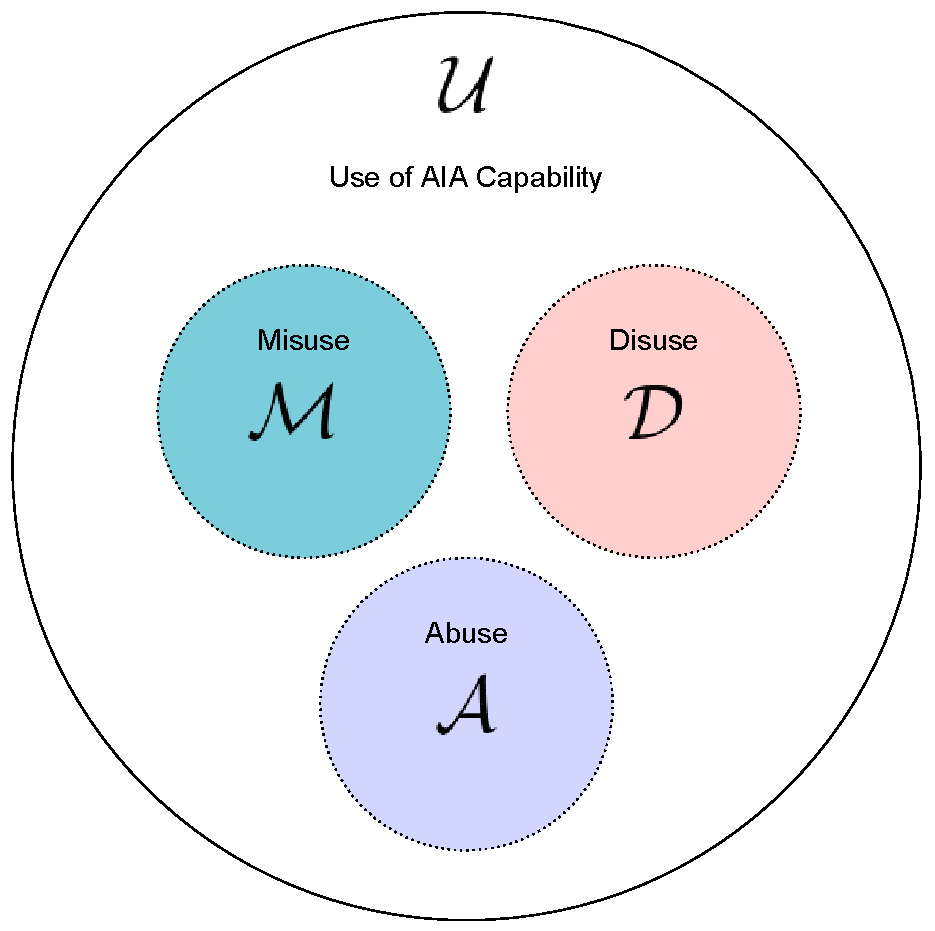
\includegraphics[width=0.4\textwidth]{Figures/misuse_disuse_abuse}
        % \caption{Graphic representing the total space of user actions, in which the inappropriate uses $\mathcal{M}$, $\mathcal{D}$, and $\mathcal{A}$ lie. The set of inappropriate uses $\mathcal{I}$ is the union of $\mathcal{M}$, $\mathcal{D}$, and $\mathcal{A}$. The appropriate set of actions $\mathcal{U}$ is the compliment of $\mathcal{I}$, or the part of $\mathcal{T}$ that does not include $\mathcal{I}$.}
        % \label{fig:appropriate_use}
    % \end{figure}
    
    Given this definition, in order to ensure that humans use AIAs appropriately, it is critical that the user TRBs be calibrated to elicit behaviors that are within the set of appropriate behaviors, which can only be done by influencing the user trust. This is a point that, to some extent, has been informally mentioned in \citet{Muir1994-ow,Muir1987-mk,Lillard2016-yg,Lee2004-pv,Hutchins2015-if}.

    A critical oversight of other researchers who mention `calibration' is that they suggest calibrating \emph{trust} as opposed to TRBs. \citet{Dzindolet2003-ts} studied the effect of performance feedback on user's self-reported trust, and found that it increased, however the appropriate TRBs toward the system didn't reflect the level of self-reported trust. This shows the danger of calibrating ``trust'', as opposed to calibrating the TRBs.

    Calibrating TRBs focuses on concrete and measurable behaviors that are universally applicable. In contrast, calibrating trust involves influencing a quantify that is directly immeasurable, and that, when measured indirectly, is subject to the biases, uncertainties, and fundamental differences of humans. Viewing the task from this point of view, the findings of \citeauthor{Dzindolet2003-ts} are not surprising.

    % \textbf{I'd like to go off on a little rant about this, but I'm not sure if it is appropriate. There is a TON of literature that talks about calibrating trust. Calibrating trust is asking for trouble, when we actually care about TRBs. VERY LITTLE RESEARCH  (none?) HAS BEEN DONE CONSIDERING ONLY TRBS, IT IS MOSTLY JUST SELF-REPORTED TRUST, WHICH DZINDOLET HAS SHOWN TO BE SHAKY GROUND} \nisarcomm{This is a very interesting point -- definitely worth mentioning as a conclusion/takeaway of this survey and worth restating/discussing in a bit more detail at the end for open opportunities and future work, etc.}

    It is desirable for AIAs to be designed in order to encourage appropriate TRBs, as opposed to the alternative of purposefully misleading users misuse or abuse. There is a valid argument that many of today's AIAs that ignore (or whose designers ignored) TRBs and assurances can be unwittingly malicious in that they do not actively attempt to guide user's TRBs to lay within the space of appropriate TRBs.
    % A benevolent AIA the user's TRBs should be appropriate \nisarcomm{I am not sure what you mean here -- when I read this sentence out loud, it doesn't really come together: what do you mean by the `perspective of a benevolent AIA'?? Also, `benevolent AIA' seems to ascribe some sort of intentionality to an AIA, which was not really discussed or mentioned at all before in your AIA definition}.
    % This in contrast to a malicious AIA that tries to manipulate the TRBs of a human to overlap with misuse, \edit{abuse} or disuse to some extent \nisarcomm{again, unclear what precisely you mean here when reading this out loud -- are you trying to make the point that simply getting a user to trust a system more is not meaningful or beneficial on its own, since it's not hard to dupe people into trusting something that's actually bad for them? (note this doesn't necessarily square with the idea you seem to be proposing of `tricking' people into abusing, misusing, or disusing AIAs -- the connotation of abuse, misuse and disuse is more that these are tendencies that people tend to converge to on their own; misuse is arguably the only one that people might actually get actively tricked into in terms of having their trust levels being actively manipulated by an AIA; interestingly, disuse can also arise in `neutral/benevolent' systems, e.g. the Mars Rovers: disuse of the advanced features onboard the rovers arises due to cultural influences at NASA, i.e. don't let rovers make decisions that can't be backtracked or accounted for fully, since the cost of failure is too high and thus the engineers are highly risk averse -- the rover autonomy itself arguably plays no role in shaping this disuse}. There is a valid argument that many of today's systems that ignore TRBs and assurances are unwittingly malicious in that they do not actively attempt to guide user's TRBs to lay within the space of appropriate TRBs .

    % Generally trust between a human and AI could be depicted as in Figure \ref{fig:SimpleTrust_two_way}, where each has TRBs that must be calibrated, and each provides certain feedback, which will be called assurances, in order to do so. In a more simple scenario, where the AI implicitly trusts the human user the trust relationship can be depicted as shown in Figure \ref{fig:SimpleTrust_one_way}, where only the user has TRBs that are being calibrated.

	% \begin{figure*}[htbp]
        % \centering
        % \begin{subfigure}[t]{0.48\textwidth}
            % \centering
            % 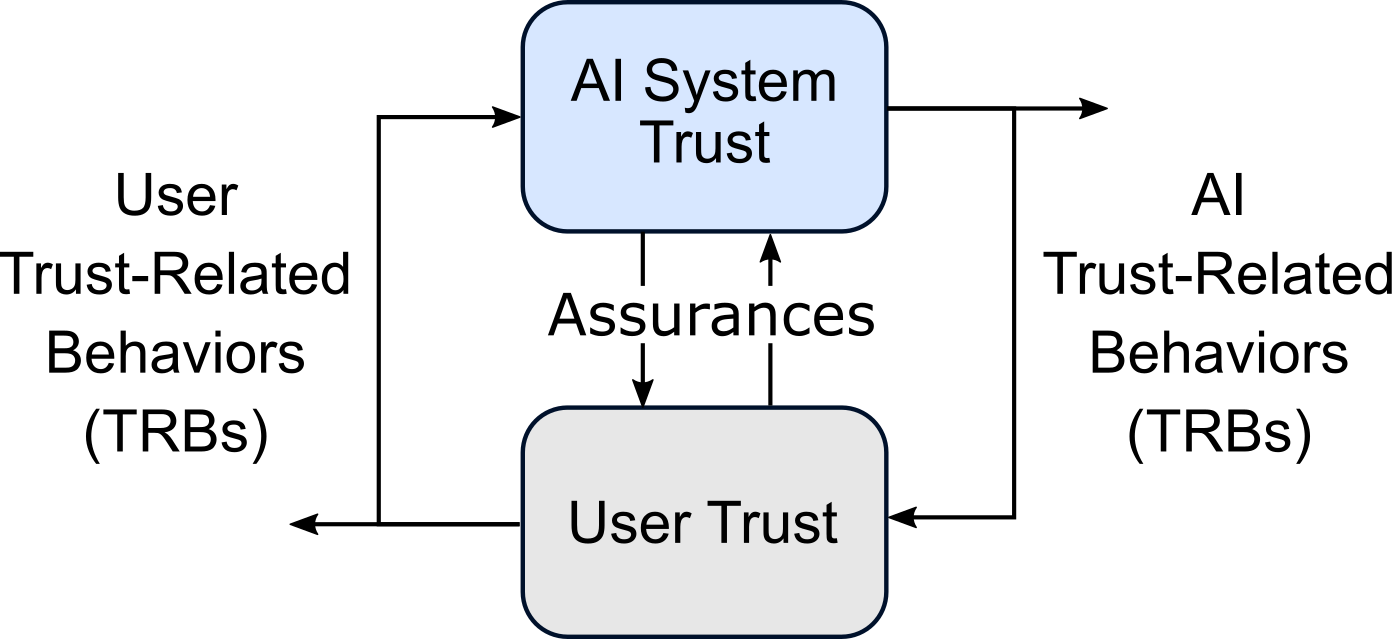
\includegraphics[width=0.95\textwidth]{Figures/SimpleTrust_two_way}
            % \caption{Diagram showing a general case of a two-way trust relationship between an AI and a human. Arrows that are not connected to boxes represent some action outside of the trust loop.}
            % \label{fig:SimpleTrust_two_way}%
        % \end{subfigure}
        % \hfill
        % \begin{subfigure}[t]{0.48\textwidth}
            % \centering
            % 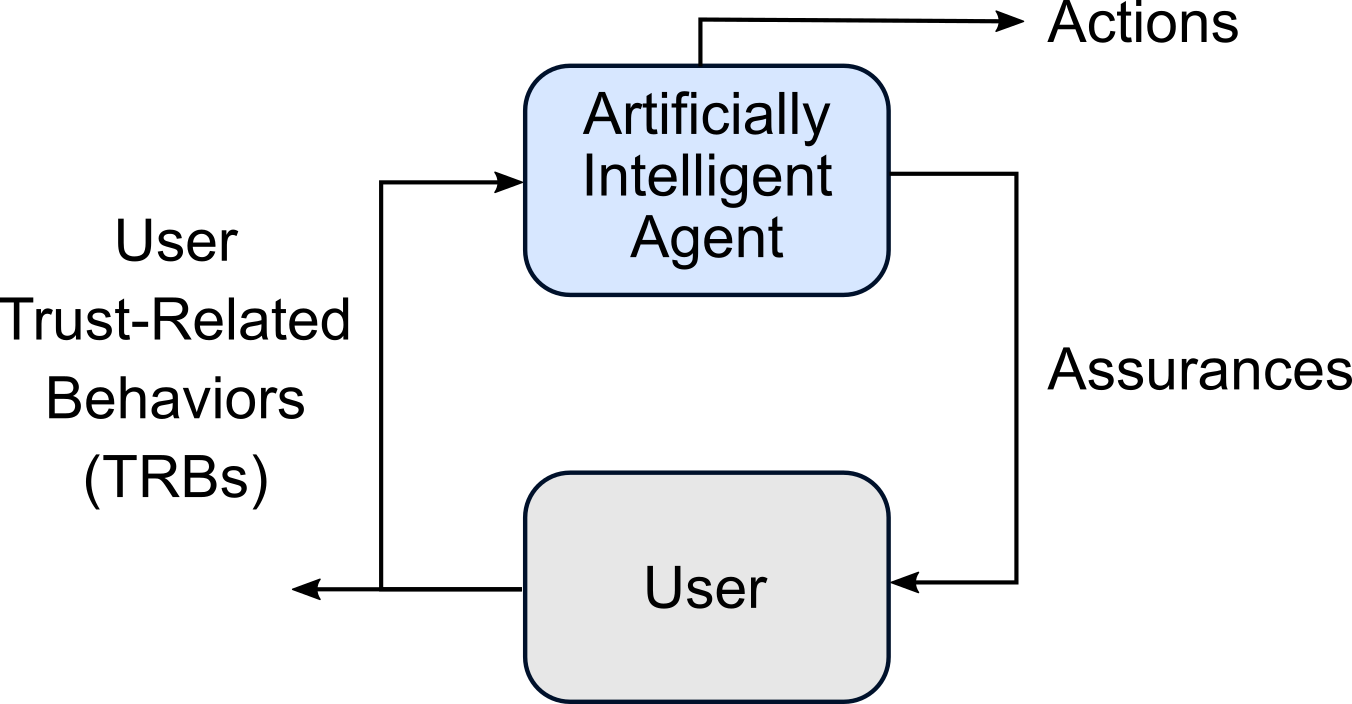
\includegraphics[width=0.95\textwidth]{Figures/SimpleTrust_one_way}
            % \caption{Diagram illustrating a general one-way trust relationship between a human and an AI. In this case the AI has, what could be considered perfect trust in the user.}
            % \label{fig:SimpleTrust_one_way}%
        % \end{subfigure}
        % \caption{Feedback Loops For One and Two-way human-AI Trust Relationships}
        % \label{fig:SimpleTrust}
    % \end{figure}
    
    % Figure \ref{fig:SimpleTrust_dist} serves as a simple example illustrating the possible disparity between the user TRB distribution and the appropriate TRB distribution. In this case assurances would be used to minimize the difference between the two distributions.

	% \begin{figure}[htbp]
        % \centering
         % 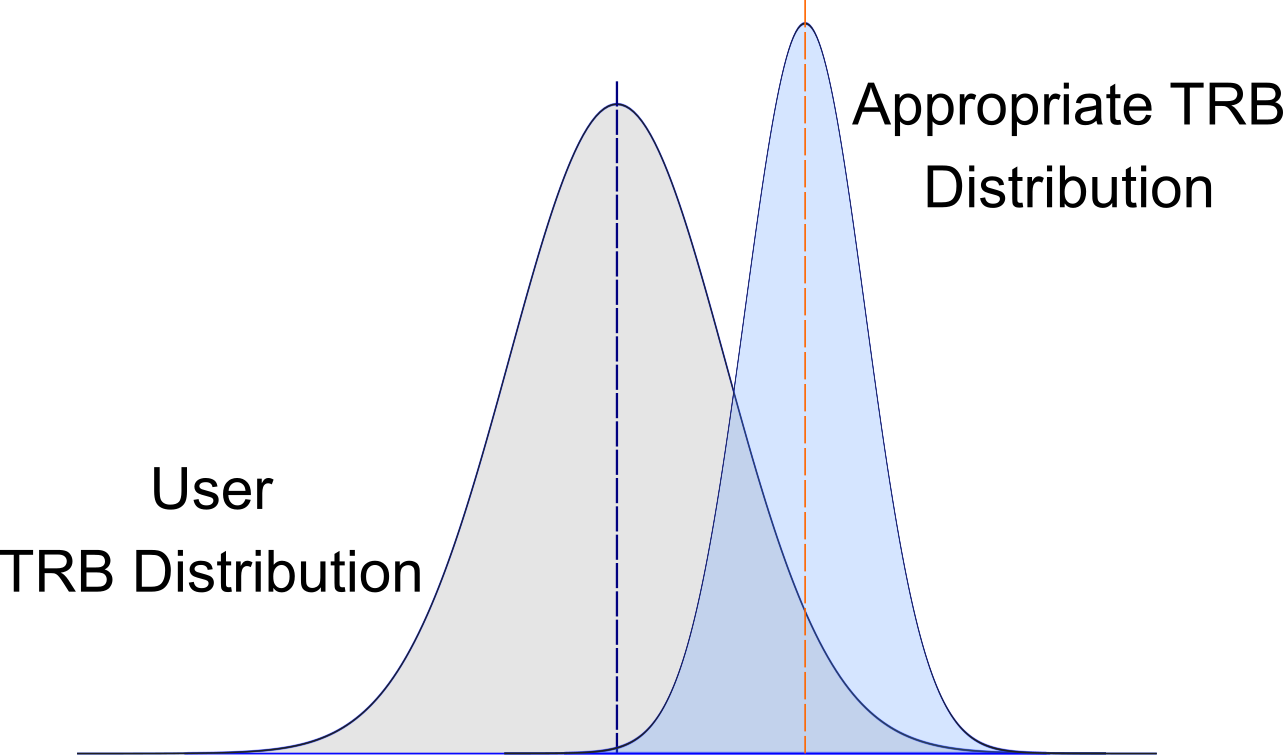
\includegraphics[width=0.4\textwidth]{Figures/SimpleTrust_dist.png}
        % \caption{Diagram illustrating the point that a hypothetical user TRB distribution might not match the appropriate TRB distribution. In this case the AI should provide assurances in order to minimize the difference between the two.}
        % \label{fig:SimpleTrust_dist}
    % \end{figure}
%
